\documentclass[a4paper,11pt]{report}
\usepackage[showexo=true,showcorr=false]{../packages/coursclasse}
%Commenter ou enlever le commentaire sur la ligne suivante pour montrer le niveau
\toggletrue{montrerNiveaux}
%permet de gérer l'espacement entre les items des env enumerate et enumitem
\usepackage{enumitem}
\setlist[enumerate]{align=left,leftmargin=1cm,itemsep=10pt,parsep=0pt,topsep=0pt,rightmargin=0.5cm}
\setlist[itemize]{align=left,labelsep=1em,leftmargin=*,itemsep=0pt,parsep=0pt,topsep=0pt,rightmargin=0cm}
%permet de gerer l'espacement entre les colonnes de multicols
\setlength\columnsep{35pt}
% \usepackage{psfrag}
% \usepackage{auto-pst-pdf}

%\usepackage[process=all]{pstool}

\begin{document}
%%%%%%%%%%%%%%%%% À MODIFIER POUR CHAQUE SERIE %%%%%%%%%%%%%%%%%%%%%%%%%%%%%
\newcommand{\chapterName}{Nombres et opérations}
\newcommand{\serieName}{Les quatre opérations}


%%%%%%%%%%%%%%%%%% PREMIERE PAGE NE PAS MODIFER %%%%%%%%%%%%%%%%%%%%%%%%
% le chapitre en cours, ne pas changer au cours d'une série
\chapter*{\chapterName}
\thispagestyle{empty}

%%%%% LISTE AIDE MEMOIRE %%%%%%
\begin{amL}{\serieName}{
\item Addition (page 22)
\item Additionner des nombres décimaux positifs en colonnes (page 23)
\item Soustraction (page 23)
\item Soustraire des nombres décimaux positifs en colonnes (page 23)
\item Multiplication (page 24)
\item Multiplier des nombres décimaux positifs en colonnes (page 24)
\item Division (page 24)
\item Diviser des nombres décimaux positifs en colonnes (page 25)
}
\end{amL}
%%%%%%%%%%%%%%% DEBUT DE LA SERIE NE PAS MODIFIER %%%%%%%%%%%%%%%%%%%%%%%%%%%%%
\section*{\serieName}
\setcounter{page}{1}
\thispagestyle{firstPage}



%%%%%%%%%%% LES EXERCICES %%%%%%%%%%%%%%%%%%%%%%%%%%%%%%%%%%%


\begin{resolu}{Vocabulaire sur les opérations}
{Complète à l'aide du vocabulaire suivant :
\begin{center}
\fbox{{\color{blue} différence}} $\quad$ \fbox{{\color{blue} dividende}} $\quad$ \fbox{{\color{blue} terme}} $\quad$ \fbox{{\color{blue} somme}} $\quad$
\end{center}
\begin{center}
\fbox{{\color{blue} facteur}} $\quad$
\fbox{{\color{blue} produit}} $\quad$
\fbox{{\color{blue} diviseur}} $\quad$
\fbox{{\color{blue} quotient}} $\quad$
\end{center}

\begin{minipage}{0.45\linewidth}
\begin{center}
\begin{psfrags}
\psfrag{A}[c][t]{5}
\psfrag{B}[c][t]{+}
\psfrag{C}[c][t]{3}
\psfrag{D}[c][t]{=}
\psfrag{E}[c][t]{8}
\psfrag{F}[c][c]{{\color{blue} terme}}
\psfrag{G}[c][c]{{\color{blue} terme}}
\psfrag{H}[c][c]{{\color{blue} somme}}
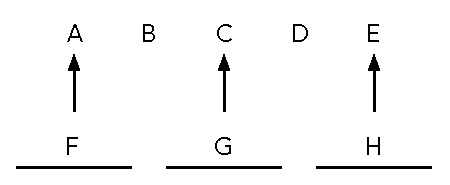
\includegraphics[scale=1]{media/no-30/vocabulaire4op.eps}
\end{psfrags}
\end{center}
\end{minipage}
\hfill
\begin{minipage}{0.45\linewidth}
\begin{center}
\begin{psfrags}
\psfrag{A}[c][t]{5}
\psfrag{B}[c][t]{$\cdot$}
\psfrag{C}[c][t]{3}
\psfrag{D}[c][t]{=}
\psfrag{E}[c][t]{15}
\psfrag{F}[c][c]{{\color{blue} facteur}}
\psfrag{G}[c][c]{{\color{blue} facteur}}
\psfrag{H}[c][c]{{\color{blue} produit}}
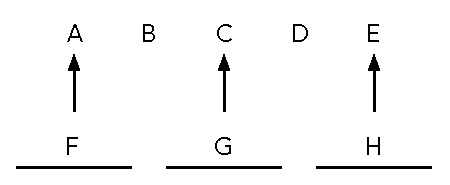
\includegraphics[scale=1]{media/no-30/vocabulaire4op.eps}
\end{psfrags}
\end{center}
\end{minipage}

\bigskip

\begin{minipage}{0,45\linewidth}
\begin{center}
\begin{psfrags}
\psfrag{A}[c][t]{5}
\psfrag{B}[c][t]{-}
\psfrag{C}[c][t]{3}
\psfrag{D}[c][t]{=}
\psfrag{E}[c][t]{2}
\psfrag{F}[c][c]{{\color{blue} terme}}
\psfrag{G}[c][c]{{\color{blue} terme}}
\psfrag{H}[c][c]{{\color{blue} différence}}
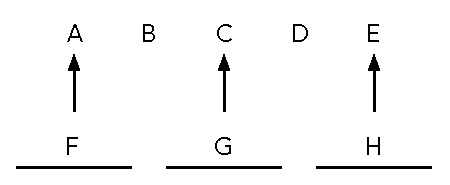
\includegraphics[scale=1]{media/no-30/vocabulaire4op.eps}
\end{psfrags}
\end{center}
\end{minipage}
\hfill
\begin{minipage}{0,45\linewidth}
\begin{center}
\begin{psfrags}
\psfrag{A}[c][t]{15}
\psfrag{B}[c][t]{ : }
\psfrag{C}[c][t]{3}
\psfrag{D}[c][t]{=}
\psfrag{E}[c][t]{5}
\psfrag{F}[c][c]{{\color{blue} dividende}}
\psfrag{G}[c][c]{{\color{blue} diviseur}}
\psfrag{H}[c][c]{{\color{blue} quotient}}
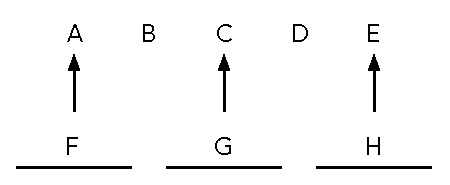
\includegraphics[scale=1]{media/no-30/vocabulaire4op.eps}
\end{psfrags}
\end{center}
\end{minipage}
}{1}
\end{resolu}

\begin{exop}{
Complète à l'aide du vocabulaire suivant :
\begin{center}
\fbox{{\color{blue} différence}} $\quad$ \fbox{{\color{blue} dividende}} $\quad$ \fbox{{\color{blue} terme}} $\quad$ \fbox{{\color{blue} somme}} $\quad$
\end{center}
\begin{center}
\fbox{{\color{blue} facteur}} $\quad$
\fbox{{\color{blue} produit}} $\quad$
\fbox{{\color{blue} diviseur}} $\quad$
\fbox{{\color{blue} quotient}} $\quad$
\end{center}

\begin{minipage}{0,45\linewidth}
\begin{center}
\begin{psfrags}
\psfrag{A}[c][t]{27}
\psfrag{B}[c][t]{-}
\psfrag{C}[c][t]{9}
\psfrag{D}[c][t]{=}
\psfrag{E}[c][t]{18}
\psfrag{F}[c][c]{{{{\color{blue} }}}}
\psfrag{G}[c][c]{{{{\color{blue} }}}}
\psfrag{H}[c][c]{{{{\color{blue} }}}}
%\psfrag{F}[c][c]{{{{\color{blue} terme}}}}
%\psfrag{G}[c][c]{{{{\color{blue} terme}}}}
%\psfrag{H}[c][c]{{{{\color{blue} différence}}}}
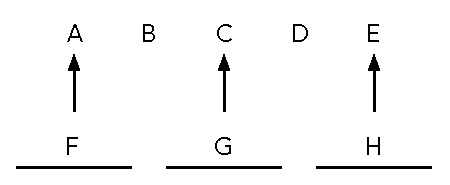
\includegraphics[scale=1]{media/no-30/vocabulaire4op.eps}
\end{psfrags}
\end{center}
\end{minipage}
\hfill
\begin{minipage}{0,45\linewidth}
\begin{center}
\begin{psfrags}
\psfrag{A}[c][t]{27}
\psfrag{B}[c][t]{+}
\psfrag{C}[c][t]{9}
\psfrag{D}[c][t]{=}
\psfrag{E}[c][t]{36}
\psfrag{F}[c][c]{{{{\color{blue} }}}}
\psfrag{G}[c][c]{{{{\color{blue} }}}}
\psfrag{H}[c][c]{{{{\color{blue} }}}}
%\psfrag{F}[c][c]{{{{\color{blue} terme}}}}
%\psfrag{G}[c][c]{{{{\color{blue} terme}}}}
%\psfrag{H}[c][c]{{{{\color{blue} somme}}}}
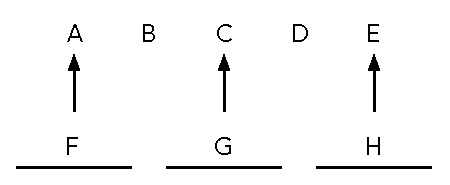
\includegraphics[scale=1]{media/no-30/vocabulaire4op.eps}
\end{psfrags}
\end{center}
\end{minipage}



\bigskip
\begin{minipage}{0,45\linewidth}
\begin{center}
\begin{psfrags}
\psfrag{A}[c][t]{27}
\psfrag{B}[c][t]{$\cdot$}
\psfrag{C}[c][t]{9}
\psfrag{D}[c][t]{=}
\psfrag{E}[c][t]{243}
\psfrag{F}[c][c]{{{{\color{blue} }}}}
\psfrag{G}[c][c]{{{{\color{blue} }}}}
\psfrag{H}[c][c]{{{{\color{blue} }}}}
%\psfrag{F}[c][c]{{{{\color{blue} facteur}}}}
%\psfrag{G}[c][c]{{{{\color{blue} facteur}}}}
%\psfrag{H}[c][c]{{{{\color{blue} produit}}}}
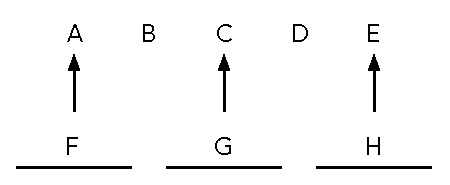
\includegraphics[scale=1]{media/no-30/vocabulaire4op.eps}
\end{psfrags}
\end{center}
\end{minipage}
\hfill
\begin{minipage}{0,45\linewidth}
\begin{center}
\begin{psfrags}
\psfrag{A}[c][t]{27}
\psfrag{B}[c][t]{ : }
\psfrag{C}[c][t]{9}
\psfrag{D}[c][t]{=}
\psfrag{E}[c][t]{3}
\psfrag{F}[c][c]{{{{\color{blue} }}}}%\psfrag{F}[c][c]{{{{\color{blue} dividende}}}}
\psfrag{G}[c][c]{{{{\color{blue} }}}}%\psfrag{G}[c][c]{{{{\color{blue} diviseur}}}}
\psfrag{H}[c][c]{{{{\color{blue} }}}}
%\psfrag{H}[c][c]{{{{\color{blue} quotient}}}}
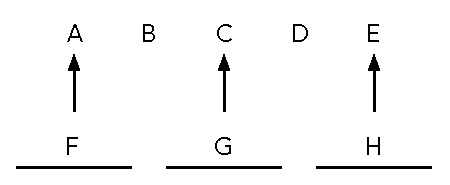
\includegraphics[scale=1]{media/no-30/vocabulaire4op.eps}
\end{psfrags}
\end{center}
\end{minipage}}{1}
\end{exop}



\begin{resolu}{Additions et soustractions}
{Effectue les additions et soustractions suivantes :
\begin{tasks}(2)
\task $709,\,48 + 57,\,9 =$ {{{\color{blue}767,38}}}
\task $303 - 98,6 =$ {{{\color{blue}204,4}}}
\task $709,\,48 - 57,\,9 =$ {{{\color{blue}651,58}}}
\task $303 + 98,6 =$ {{{\color{blue}401,6}}}
\end{tasks}
\begin{minipage}{0,45\linewidth}
{{{\color{blue}
\begin{tabular}{ccccccc}
& & {\color{red}\footnotesize{1}} & {\color{red}\footnotesize{1}}& & & \\
&7&0&9& , &4 & 8 \\
${\color{blue}+}$&  &5 & 7 & , & 9 & 0 \\\hline
 & 7& 6& 7& ,& 3&8
\end{tabular} }}}
\end{minipage} \hfill
\begin{minipage}{0,45\linewidth}
{{{\color{blue}
\begin{tabular}{cccccc}
& & {\color{red}\footnotesize{9}} & {\color{red}\footnotesize{12}} & & \\
& {\color{red}\footnotesize{2}} & {\bcancel{\color{red}\footnotesize{10}}} &{\bcancel{\color{red}\footnotesize{2}}} & & {\color{red}\footnotesize{10}} \\
&\cancel{3} &\cancel{0} &\xcancel{3} &, & 0 \\
${\color{blue}-}$& &9  & 8& , & 6 \\\hline
& 2 & 0 & 4 &, & 4 
\end{tabular}
 }}}
\end{minipage}

\bigskip

\begin{minipage}{0,45\linewidth}
{{{\color{blue}
\begin{tabular}{ccccccc}
& {\color{red}\footnotesize{6}} & {\color{red}\footnotesize{10}} & {\color{red}\footnotesize{8}}& & {\color{red}\footnotesize{14}} & \\
&\cancel{7}&\bcancel{0}&\cancel{9}& , &\bcancel{4} & 8 \\
${\color{blue}-}$&  &5 & 7 & , & 9 & 0 \\\hline
 & 6& 5& 1& ,& 5&8
\end{tabular}
 }}}
\end{minipage} \hfill
\begin{minipage}{0,45\linewidth}
{{{\color{blue}
\begin{tabular}{cccccc}
&{\color{red}\footnotesize{1}} & {\color{red}\footnotesize{1}} & & & \\
&3&0&3& , & 0 \\
${\color{blue}+}$ & & 9& 8 & , & 6 \\\hline
&4 & 0 & 1 & , &6 
\end{tabular} }}}
\end{minipage}
}{1}
\end{resolu}

\begin{exop}{
Effectue les additions suivantes :
\bigskip
\begin{tasks}(2)
\task {{
\begin{tabular}{cccc}
& 6& 9& 7  \\
$+$ &7 & 8& 8 \\\hline
\end{tabular} }}
\task {{
\begin{tabular}{ccccc}
& 2&1 &6 & 2  \\
$+$ &1 &2 & 6& 4    \\\hline
\end{tabular} }}
\end{tasks}
\vspace*{1cm}}{1}
\end{exop}

\begin{exop}{
Effectue les additions suivantes :
\bigskip
\begin{tasks}(2)
\task {{
\begin{tabular}{cccccc}
& & 4& 5& , & 0 \\
$+$ & 2& 0 &7 & ,& 9  \\\hline
\end{tabular} }}
\task {{
\begin{tabular}{ccccccc}
&2& 3& 6& 5&, & 7 \\
	$+$ &&1 & 5& 6&, & 3  \\\hline
\end{tabular} }}
\end{tasks}
\vspace*{1cm}}{1}
\end{exop}


\begin{exop}{
Effectue les additions suivantes :
\bigskip
\begin{tasks}(2)
\task {{
\begin{tabular}{ccccccc}
&2&5&7& , & 9&2 \\
$+$ & 3&7&5&,&0&9 \\\hline
\end{tabular} }}
\task {{
\begin{tabular}{ccccccc}
&3&9&2& , & 5&8 \\
$+$ & 1&6&9&,&1&4 \\\hline
\end{tabular} }}
\end{tasks}
\vspace*{1cm}}{1}
\end{exop}


\begin{exop}{
Effectue les soustractions suivantes :
\bigskip
\begin{tasks}(2)
\task {{
\begin{tabular}{cccc}
&9 &2 &5  \\
$-$ & 7& 5&2  \\\hline
\end{tabular} }}
\task {{
\begin{tabular}{ccccc}
&7&5 &9 &4  \\
$-$ &&6 &2 &6   \\\hline
\end{tabular} }}
\end{tasks}
\vspace*{1cm}
}{1}\end{exop}

\begin{exop}{
Effectue les soustractions suivantes :
\bigskip
\begin{tasks}(2)
\task {{
\begin{tabular}{ccccc}
&9 & 4& ,&9   \\
	$-$ &6 &3 &, &5  \\\hline
\end{tabular} }}
\task {{
\begin{tabular}{cccccc}
&1& 2&3 &, & 6 \\
$-$& & 6& 7&, & 8  \\\hline
\end{tabular} }}
\end{tasks}
\vspace*{1cm}
}{1}\end{exop}

\begin{exop}{
Effectue les soustractions suivantes :
\bigskip
\begin{tasks}(2)
\task {{
\begin{tabular}{ccccccc}
&1 & 5& 0& , &0 & 8 \\
$-$ & & 4&6 &, &1 &7 \\\hline
\end{tabular} }}
\task {{
\begin{tabular}{ccccccc}
& 5& 6& 8& ,& 6& 0 \\
$-$ &2 &4 &8 &, &9 & 5  \\\hline
\end{tabular} }}
\end{tasks}
\vspace*{1cm}
}{1}\end{exop}


\begin{resolu}{Multiplications}
{Effectue les multiplications suivantes :
\begin{tasks}(2)
\task $5,6 \cdot 87 =$ {{{\color{blue}487,2}}}
\task $5,6 \cdot 8,7 =$ {{{\color{blue}48,72}}}
\task $102 \cdot 35 =$ {{{\color{blue}3570}}}
\task $1,02 \cdot 3,5 =$ {{{\color{blue}3,57}}}
\end{tasks}

\bigskip

\begin{minipage}{0,45\linewidth}
{{{\color{blue}
\begin{tabular}{ccccc}
 & & {\color{red}\footnotesize{4}} &{\color{red}\footnotesize{4}} & \\
 & & {\color{red}\footnotesize{3}} & {\color{red}\footnotesize{4}} & \\
 & & & 5, & 6 \\
  & &${\color{blue}\cdot}$ & 8 & 7 \\\hline
   & & {\color{red}\footnotesize{1}} & & \\
  & & 3 & 9 & 2 \\ 
${\color{blue}+}$ & 4 & 4 & 8 & 0\\\hline
& 4 & 8 & 7, &2 \\
\end{tabular}
}}}
\end{minipage}\hfill
\begin{minipage}{0,45\linewidth}
{{{\color{blue}
\begin{tabular}{ccccc}
 & & {\color{red}\footnotesize{4}} &{\color{red}\footnotesize{4}} & \\
 & & {\color{red}\footnotesize{3}} & {\color{red}\footnotesize{4}} & \\
 & & & 5, & 6 \\
  & & ${\color{blue}\cdot}$& 8, & 7 \\\hline
   & & {\color{red}\footnotesize{1}} & & \\
  & & 3 & 9 & 2 \\ 
${\color{blue}+}$ & 4 & 4 & 8 & 0\\\hline
& 4 & 8, & 7 &2 \\
\end{tabular}
}}}
\end{minipage}

\bigskip

\begin{minipage}{0,45\linewidth}
{{{\color{blue}
\begin{tabular}{ccccc}
& & &{\color{red}\footnotesize{1}}  & \\
& & 1 & 0 &2 \\
& & ${\color{blue}\cdot}$ & 3 & 5 \\\hline
& & 5 & 1 & 0 \\
${\color{blue}+}$ & 3 & 0 & 6 & 0 \\\hline
& 3 & 5 & 7 & 0 \\
\end{tabular}
}}}
\end{minipage}\hfill
\begin{minipage}{0,45\linewidth}
{{{\color{blue}
\begin{tabular}{ccccc}
& & &{\color{red}\footnotesize{1}}  & \\
& & 1, & 0 &2 \\
& & ${\color{blue}\cdot}$ & 3, & 5 \\\hline
& & 5 & 1 & 0 \\
${\color{blue}+}$ & 3 & 0 & 6 & 0 \\\hline
& 3, & 5 & 7 & 0 \\
\end{tabular}
}}}
\end{minipage}


}{1}
\end{resolu}

\begin{exop}{
Effectue les multiplications suivantes : 
\bigskip
\begin{tasks}(2)
\task {{
\begin{tabular}{cccccc}
& & &2&3&4 \\
$\cdot$ & & & &1&9 \\\hline \\ \\ $+$ & & & & &\\\hline  
\end{tabular} }}
\task {{
\begin{tabular}{cccccccc}
& & &2&3&,&4 \\
$\cdot$ & & & &1&,&9 \\\hline \\ \\ $+$ & & & & & &\\\hline  
\end{tabular} }}
\end{tasks}
\vspace*{1cm}
}{1}
\end{exop}

\begin{exop}{
Effectue les multiplications suivantes : 
\bigskip
\begin{tasks}(2)
\task {{
\begin{tabular}{cccccc}
& & &4&7&6 \\
$\cdot$ & & & &5&8 \\\hline \\ \\ $+$ & & & & &\\\hline  
\end{tabular} }}
\task {{
\begin{tabular}{cccccccc}
& & &4&,&7&6 \\
$\cdot$ & & & 0&,&5&8 \\\hline \\ \\ $+$ & & & & & &\\\hline  
\end{tabular} }}
\end{tasks}
\vspace*{1cm}
}{1}
\end{exop}


\begin{exop}{
Effectue les multiplications suivantes : 
\bigskip
\begin{tasks}(2)
\task {{
\begin{tabular}{cccccc}
& & &1&5&7 \\
$\cdot$ & & & &5&8 \\\hline \\ $+$ & & & & &\\\hline  
\end{tabular} }}
\task {{
\begin{tabular}{cccccccc}
& & 1&,&5&7& \\
$\cdot$ & &0 & ,&0&5&8 \\\hline \\ $+$ & & & & & &\\\hline  
\end{tabular} }}
\end{tasks}
\vspace*{1cm}
}{1}
\end{exop}




\begin{resolu}{Divisions}
{Effectue les divisions suivantes :
\begin{tasks}(3)
\task $46,32 \div 4 =11,58$
\task*(2) $\underbrace{46,32}_{\rightarrow\mbox{1 rang}} \div \underbrace{0,4}_{\rightarrow\mbox{1 rang}} =463,2 \div 4 = 115,8$
\task $25,36 \div 5 = 5,072$
\task*(2) $\underbrace{25,36}_{\rightarrow\mbox{2 rangs}} \div \underbrace{0,05}_{\rightarrow\mbox{2 rangs}} = 2536 \div 5 = 507,2$
\end{tasks}

\bigskip

\begin{minipage}{0.4\linewidth}
{{{\color{blue}
\begin{tabular}{ccccc|cccc}
&4&6,&3&2  &4 & & &  \\\cline{6-9}
${\color{blue}-}$& 4& $\downarrow$ & $\downarrow$ & $\downarrow$ & 1 & 1, & 5 &8 \\\cline{1-2}
& 0 & 6 &  $\downarrow$ & $\downarrow$  & & &  \\
& ${\color{blue}-}$& 4 & $\downarrow$ & $\downarrow$  & & & \\\cline{2-3}
& & 2 & 3 & $\downarrow$  & & & \\
& ${\color{blue}-}$ & 2 & 0  & $\downarrow$  & & & \\\cline{2-4}
&  & & 3&2  & & & & \\
& & ${\color{blue}-}$ & 3&2  & & & & \\\cline{3-5}
& & &  & 0  & & & &
\end{tabular}
}}}
\end{minipage} \hfill
\begin{minipage}{0.45\linewidth}
{{{\color{blue}
\begin{tabular}{ccccc|cccc}
&4&6&3,&2  &4 & & &  \\\cline{6-9}
${\color{blue}-}$& 4& $\downarrow$ & $\downarrow$ & $\downarrow$  & 1 & 1 & 5, &8 \\\cline{1-2}
& 0 & 6 &  $\downarrow$ & $\downarrow$  & & &  \\
& ${\color{blue}-}$& 4 & $\downarrow$ & $\downarrow$  & & & \\\cline{2-3}
& & 2 & 3 & $\downarrow$  & & & \\
& ${\color{blue}-}$ & 2 & 0  & $\downarrow$  & & & \\\cline{2-4}
&  & & 3&2  & & & & \\
& & ${\color{blue}-}$ & 3&2 & & & & \\\cline{3-5}
& & &  & 0  & & & &
\end{tabular}
}}}
\end{minipage}

\bigskip

\bigskip

\begin{minipage}{0,45\linewidth}
{{{\color{blue}
\begin{tabular}{cccccc|cccc}
&2 &5, &3 &6 & 0 &  5 & & & \\\cline{7-10}
${\color{blue}-}$ & 2 & 5 &$\downarrow$ &$\downarrow$ &$\downarrow$ &5, &0 & 7 & 2 \\\cline{1-3}
& &0 &3 &$\downarrow$ &$\downarrow$  & & & & \\
& & ${\color{blue}-}$ & 0 & $\downarrow$ & $\downarrow$  & & & & \\\cline{3-4}
& & &3 &6 & $\downarrow$  & & & & \\
& & ${\color{blue}-}$ &3 & 5 &$\downarrow$  & & & & \\\cline{3-5}
& & & & 1 & 0  & & & & \\
& & & ${\color{blue}-}$& 1 & 0  & & & & \\\cline{4-6}
& & & & & 0  & & & & \\
\end{tabular}
}}}
\end{minipage} \hfill
\begin{minipage}{0,45\linewidth}
{{{\color{blue}
\begin{tabular}{cccccc|cccc}
&2 &5 &3 &6, & 0  & 5 & & & \\\cline{7-10}
${\color{blue}-}$ & 2 & 5 &$\downarrow$ &$\downarrow$ &$\downarrow$ &5 &0 & 7, & 2 \\\cline{1-3}
& &0 &3 &$\downarrow$ &$\downarrow$  & & & & \\
& & ${\color{blue}-}$ & 0 & $\downarrow$ & $\downarrow$  & & & & \\\cline{3-4}
& & &3 &6 & $\downarrow$  & & & & \\
& & ${\color{blue}-}$ &3 & 5 &$\downarrow$  & & & & \\\cline{3-5}
& & & & 1 & 0  & & & & \\
& & & ${\color{blue}-}$& 1 & 0 & & & & \\\cline{4-6}
& & & & & 0  & & & & \\
\end{tabular}
}}}
\end{minipage}

}{1}
\end{resolu}

\begin{exop}{
Effectue les divisions suivantes :
\begin{tasks}(1)
\task $437,22 \div 6 =$
\task $\underbrace{437,22}_{\rightarrow\mbox{1 rang}} \div \underbrace{0,6}_{\rightarrow\mbox{1 rang}}=$
\end{tasks}

\bigskip

\begin{minipage}{0,45\linewidth}
\begin{tabular}{cccccc|ccccc}
4&3&7,&2&2 & &6 & & & & \\\cline{7-11}
& & & & & & & & & & \\
& & & & & & & & & & \\
& & & & & & & & & & \\
& & & & & & & & & & \\
& & & & & & & & & & \\
& & & & & & & & & & \\
& & & & & & & & & & \\
& & & & & & & & & & \\
& & & & & & & & & & \\
& & & & & & & & & & \\
\end{tabular}
\end{minipage} \hfill
\begin{minipage}{0,45\linewidth}
\begin{tabular}{cccccc|ccccc}
4&3&7&2,&2 & &6 & & & & \\\cline{7-11}
& & & & & & & & & & \\
& & & & & & & & & & \\
& & & & & & & & & & \\
& & & & & & & & & & \\
& & & & & & & & & & \\
& & & & & & & & & & \\
& & & & & & & & & & \\
& & & & & & & & & & \\
& & & & & & & & & & \\
& & & & & & & & & & \\
\end{tabular}
\end{minipage}
}{1}
\end{exop}


\begin{exop}{
Effectue les divisions suivantes :
\begin{tasks}(1)
\task $\underbrace{108,54}_{\rightarrow\mbox{1 rang}} \div \underbrace{0,9}_{\rightarrow\mbox{1 rang}}=$
\task $\underbrace{45,318}_{\rightarrow\mbox{2 rangs}} \div \underbrace{0,03}_{\rightarrow\mbox{2 rangs}}=$

\end{tasks}

\bigskip

\begin{minipage}{0,45\linewidth}
\begin{tabular}{cccccc|ccccc}
1&0&8&5,&4 & &9 & & & & \\\cline{7-11}
& & & & & & & & & & \\
& & & & & & & & & & \\
& & & & & & & & & & \\
& & & & & & & & & & \\
& & & & & & & & & & \\
& & & & & & & & & & \\
& & & & & & & & & & \\
& & & & & & & & & & \\
& & & & & & & & & & \\
& & & & & & & & & & \\
\end{tabular}
\end{minipage} \hfill
\begin{minipage}{0,45\linewidth}
\begin{tabular}{cccccc|ccccc}
4&5&3&1,&8 & &3 & & & & \\\cline{7-11}
& & & & & & & & & & \\
& & & & & & & & & & \\
& & & & & & & & & & \\
& & & & & & & & & & \\
& & & & & & & & & & \\
& & & & & & & & & & \\
& & & & & & & & & & \\
& & & & & & & & & & \\
& & & & & & & & & & \\
& & & & & & & & & & \\
\end{tabular}
\end{minipage}
}{1}
\end{exop}


\begin{exo}{
Pose et effectue les calculs suivants :
\begin{tasks}[after-item-skip = 0.4em, after-skip=-0.5em](2)
\task $127+52 =$
\task $146-32=$
\task $25\cdot 5 =$
\task $175 \div 5 =$
\end{tasks}
}{1}\end{exo}

\begin{exo}{
Pose et effectue les calculs suivants :
\begin{tasks}[after-item-skip = 0.4em, after-skip=-0.5em](2)
\task $165+41 =$
\task $290-74=$
\task $57\cdot 6 =$
\task $848 \div 8 =$
\end{tasks}
}{1}\end{exo}

\begin{exo}{
Pose et effectue les calculs suivants :
\begin{tasks}[after-item-skip = 0.4em, after-skip=-0.5em](2)
\task $218+156 =$
\task $362-76=$
\task $136\cdot 8 =$
\task $734 \div 4 =$
\end{tasks}
}{1}\end{exo}


\begin{exo}{
Pose et effectue les calculs suivants :
\begin{tasks}[after-item-skip = 0.4em, after-skip=-0.5em](2)
\task $56,3+41,6 =$
\task $84,7-2,5=$
\task $42\cdot 1,2 =$
\task $12,6 \div 6 =$
\end{tasks}
}{1}\end{exo}

\begin{exo}{
Pose et effectue les calculs suivants :
\begin{tasks}[after-item-skip = 0.4em, after-skip=-0.5em](2)
\task $31,7+8,3 =$
\task $222,2-6,5=$
\task $73\cdot 2,3 =$
\task $18,27 \div 7 =$
\end{tasks}
}{1}\end{exo}

\begin{exo}{
Pose et effectue les calculs suivants :
\begin{tasks}[after-item-skip = 0.4em, after-skip=-0.5em](2)
\task $93,4+9,8 =$
\task $65,4 -48,6=$
\task $3,2\cdot 35 =$
\task $47,5 \div 8 =$
\end{tasks}
}{1}\end{exo}

\begin{exo}{
Pose et effectue les calculs suivants :
\begin{tasks}[after-item-skip = 0.4em, after-skip=-0.5em](2)
\task $82,9+16,4 =$
\task $607-127,7=$
\task $3,7\cdot 4,2 =$
\task $51,4 \div 0,9 =$
\end{tasks}
}{1}\end{exo}

\begin{exo}{
Pose et effectue les calculs suivants :
\begin{tasks}[after-item-skip = 0.4em, after-skip=-0.5em](2)
\task $97,17+38,3 =$
\task $652,7-388=$
\task $8,4\cdot 5,06 =$
\task $429,68 \div 0,3 =$
\end{tasks}
}{1}\end{exo}

\begin{exo}{
Pose et effectue les calculs suivants :
\begin{tasks}[after-item-skip = 0.4em, after-skip=-0.5em](2)
\task $7,13+529,8 =$
\task $687,4-48,59=$
\task $36,9\cdot 3,7 =$
\task $239,2 \div 1,1 =$
\end{tasks}
}{1}\end{exo}

\begin{exo}{
Pose et effectue les calculs suivants :
\begin{tasks}[after-item-skip = 0.4em, after-skip=-0.5em](2)
\task $413,5+34,69 =$
\task $494,5-456,9=$
\task $87,6\cdot 72,3 =$
\task $227 \div 1,1 =$
\end{tasks}
}{1}\end{exo}

\begin{exo}{
Pose et effectue les calculs suivants :
\begin{tasks}[after-item-skip = 0.4em, after-skip=-0.5em](2)
\task $1072,5+257,83 =$
\task $610,7-347,33=$
\task $5,92\cdot 4,53 =$
\task $554613,2  \div 0,8 =$
\end{tasks}
}{1}\end{exo}

\begin{exo}{
Pose et effectue les calculs suivants :
\begin{tasks}[after-item-skip = 0.4em, after-skip=-0.5em](2)
\task $64+46,9+84,52 =$
\task $1059,3-774,69=$
\task $4,73\cdot 24,7 =$
\task $70,04 \div 1,2 =$
\end{tasks}
}{1}\end{exo}

\exof{NO91}{33}{1}

\exof{NO101}{38}{1}

% Exercice à ajouter sur la proposition de Christine
\exol{NO82}{28}{1}
\exol{NO83}{29}{1}

\vfill

\exof{NO92}{34}{1}

\vfill

\exof{NO93}{34}{3}

\vfill

\exof{NO98}{36}{1}

\vfill

%%%%%%%%%%%%%%%%%%%% Problèmes %%%%%%%%%%%%%%%%

%%%%%%% Problèmes de Marie %%%%%%%%%%%%%%%%

\begin{exo}{
    Pour chacun des problèmes suivants, fais un croquis qui facilitera ta réponse à la question posée, puis réponds à cette question.
    
    \begin{tasks}(1)
	    \task Une corde de \tunit{10}{\m} de long est coupée en quatre parties égales. Combien mesure une longueur~?
	    \task Kahys et Taylan pèsent ensemble \tunit{62,8}{\kg}. Taylan pèse \tunit{6}{\kg} de plus que Kahys. Quel est le poids de chacun des enfants~?
	    \task Silvia veut brûler un grand morceau de bois de \tunit{1,80}{\m} dans la cheminée. Pour cela, elle le scie en trois morceaux égaux. Quelle sera la longueur des bûches obtenues~?
	    \task Christian achète une guirlande électrique longue de \tunit{1,60}{\m}. De chaque côté, le fil ne comporte pas d'ampoules sur une longueur de \tunit{30}{\cm}. L'intervalle séparant deux ampoules étant de \tunit{10}{\cm}, de combien d'ampoules est composée cette guirlande~?
	    \task Aurélie, avec ses \tunit{30}{\fr}, achète un livre à \tunit{8,50}{\fr} et un autre à \tunit{13,20}{\fr} Quelle somme lui reste-t-il~?
    \end{tasks}
}{1}\end{exo}


\vfill

\newpage

\begin{exo}{
    Associe l'un des calculs $A, B, C$ ou $D$ à chacun des trois problèmes. Puis, donne les réponses aux problèmes. 
    \vspace{-0.5cm}
    \begin{center}
    \begin{multicols}{2}
    $A=5\cdot(4+8)$ \\
    $B=4+5\cdot8$\quad~ \\
    $C=5+4\cdot8$\quad~ \\
    $D=5\cdot4+5\cdot8$
    \end{multicols}
    \end{center}
    
    \begin{enumerate}
	    \item[\ligne{2}] Fanny achète un livre à \tunit{4}{\fr} et cinq bandes dessinées à \tunit{8}{\fr} l'unité. Combien paie-t-elle~?
	    \item[\ligne{2}] Laure prépare cinq bouquets qui auront chacun quatre roses blanches et huit roses rouges. Combien lui faut-il de roses~?
	    \item[\ligne{2}]  À la cantine, il y a quatre tables de huit et une table de cinq. Combien de places y a-t-il au total~?
    \end{enumerate}
    
}{1}\end{exo}

\begin{exo}{
    Associe l'un des calculs $A, B, C$ ou $D$ à chacun des trois problèmes. Puis, donne les réponses aux problèmes.
    \vspace{-0.5cm}
    \begin{center}
    \begin{multicols}{2}
    $A=3\cdot0,50+1,60$ \\
    $B=3\cdot1,60+0,50$ \\
    $C=3\cdot(1,60+0,50)$ \\
    $D=3\cdot1,60+3\cdot0,50$    
    \end{multicols}
    \end{center}
    
    \begin{enumerate}
	    \item[\ligne{2}] Pollux achète trois stylos à \tunit{1,60}{\fr} l'unité et une règle à \tunit{0,50}{\fr} Combien paie-t-il~?
	    \item[\ligne{2}] Maël achète à chacun de ses trois enfants un stylo à \tunit{1,60}{\fr} et une règle à \tunit{0,50}{\fr} Combien paie-t-il~? 
	    \item[\ligne{2}] Mira a \tunit{1,60}{\fr} dans son porte-monnaie. Trois de ses amies lui remboursent chacune la somme de \tunit{0,50}{\fr} À présent, combien d'argent a Mira dans son porte-monnaie~?
    \end{enumerate}
    
}{1}\end{exo}





\exol{NO85}{29}{1}
\exol{NO86}{30}{2}
\exol{NO87}{30}{1}
\exol{NO88}{30}{1}
\exof{NO96}{35}{1}
\exof{NO97}{36}{2}





\end{document}
